\cotefile{136}
\scanpage{312}
\mspage{11}
% archive sheet number: 313

la seule connaissance de $C_{\cdot}\in\mathit{Ab}_{\cdot}$, au lieu
et place de $X_{\ast}$ ; il faut, pour \deleted{\unsure{le transport|le transfert}} 
décrire en \uline{termes de} $C_{\cdot}$ \deleted{en} \inserted{certaines des} structures
qu'on peut \inserted{ainsi} décrire sur $F(X_{\ast})$, en termes
de celles de $F$, de tenir compte des
structures supplémentaires convenables
de $C_{\cdot}$, qui peuvent s'expliciter en se
rappelant que $C_{\cdot}$ provient d'un $X_{\ast}$. \deleted{\unsure{Que}}
L'étude systématique de ces structures \deleted{\unsure{qui}}
\deleted{est} \inserted{peut être considéré comme} le contenu essentiel de ces réflexions.

Mais bien sûr, \deleted{si les structures} \inserted{dans les} \unsure{cas} disons
où on a sur $F$ une structure de
$k$-module, i.e. $F:\unsure{\mathscr S|\mathit{Se}|\mathcal{S}s}^{\circ}\unsure{\mathbin{-}|\longrightarrow}\mathit{Ab}_k$
(où $\mathit{Ab}_k$ est la catégorie des $k$-modules),
\deleted{il suffit} \inserted{il est inutile} de se donner de structure
suppl. sur $C^{\unsure{\cdot|\circ|.}}$, car \deleted{\unsure{tous}} grâce au \deleted{fait}
\deleted{\unsure{de compléter par des|d'employer des|de complexe de} $k$-chaînes sur $C_{\cdot}$
(i.e. se donner $k\longrightarrow\operatorname{End}_{\mathit{Ab}_{\cdot}}(C_{\cdot})$ pour
récupérer la structure complète de}
que le $K_{\cdot}$ qui décrit $F$ est
maintenant dans $(\mathit{Ab}_k)_{\cdot}$ i.e. qu'on a

\[
k\longrightarrow\operatorname{End}_{\mathit{Ab}_{\cdot}}(K_{\cdot})
\]

$k$ opère aussi sur $\operatorname{Hom}_{\mathit{Ab}_{\cdot}}(C_{\cdot},K_{\cdot})$,
dont on récupère ainsi la structure
de $k$-module. En \deleted{fait,} il suffit,
au lieu de $C_{\cdot}$, de \unsure{connaitre|connaître}
seulement $\inserted{C_{\unsure{k\ast k|k\ast|k\cdot}}=}C_{\cdot}\otimes_{\mathbb Z} k$ (noté $\mathbb C_{k\ast}(X_{\ast})$),
car on aura

\deleted{\unsure{les relations}}
\[
\left\{\begin{aligned}
F(X_{\ast})&\simeq\operatorname{Hom}_{(\mathit{Ab}_k)_{\cdot}}(C_{k\cdot},K_{\cdot})\\
C_{k\cdot}&=\mathbb C_{k\ast}(X_{\ast})=\mathbb C_{\ast}(X_{\ast})\otimes_{\mathbb Z} k
\end{aligned}\right.
\]

Plus généralement, revenant au cas d'une
$B$ cat. additive générale stable par $\varprojlim$
et $F:(\mathrm{\unsure{Se|S|Ss}}_{\mathrm{f}\unsure{.}})^{\circ}\longrightarrow B$ et $K_{\cdot}\in B_{\cdot}$ se correspondant par la prop. 2, on peut encore
écrire
\[
F(X_{\ast})\simeq\operatorname{Hom}_{\cdot\deleted{\unsure{B}}}^{\unsure{\circ|0|\cdot}}(\mathbb C_{\cdot}(X_{\ast}),K_{\cdot})
\]

en définissant le deuxième mb comme
\uline{objet de $B$}, en définissant d'abord le
bicomplexe de $B$
\[
\begin{aligned}
\mathcal{H}\mathrm{om}^{\cdot}_{\cdot}(C_{\cdot},K_{\cdot})&=
\bigl(\operatorname{Hom}_{B}(C_i,K_j)\bigr)_{i,j}\\
\text{(donc}\qquad \mathcal{H}\mathrm{om}^{i}_{j}(C_{\cdot},K_{\cdot})&=
\operatorname{Hom}_{B}(C_i,K_j)) 
\end{aligned}
\]

-- où l'objet $\mathrm{Hom}(A,M)$, pour $A\in\mathit{Ab}$
et $M\in B$, se définissant par
\[
\operatorname{Hom}_{\uline{B}}(N,\mathrm{Hom}(A,M))\simeq
\operatorname{Hom}_{\mathit{Ab}}(A,\operatorname{Hom}_{B}(N,M))
\]
(le foncteur \deleted{étant \unsure{repr.}} \inserted{du $2^{\text{ème}}$ mb} étant bien
représentable en $N$, pour $A,M$ fixés, grâce
à l'hyp. faite sur $B$ d'être stable par $\varprojlim$).

On définit alors
\[
\operatorname{Hom}_{\cdot}(\mathbb C_{\cdot},\deleted{\unsure{X_{\ast}}},K_{\cdot})
\overset{\mathrm{défn}}{=} Z^0(\mathcal{H}\mathrm{om}^{\cdot}_{\cdot}(\mathbb C_{\cdot},K_{\cdot}))
\]
\inserted{cycles de degré 0 pour degré total (\unsure{cohomol.|contrav.|associé} bien \unsure{ent.}).}

Si enfin $B$ est une cat. $k$-linéaire
($k$ commut.\ \unsure{tjs}) i.e. munie d'un hom d'
anneaux $k\longrightarrow\operatorname{End}(\mathrm{id}_{\uline{B}})$,

\scanpage{313}
\mspage{12}
% archive sheet number: 314

Alors la connaissance de $C_{\cdot\deleted{\unsure{\ast}}}=\mathbb C_{k\cdot}(X_{\ast})
=\mathbb C_{\cdot}\otimes_{\mathbb Z}k$ est encore suffisante pour
la construction de $F(X_{\ast})$, car on aura
maintenant
\[
\begin{aligned}
F(X_{\ast})&\simeq\operatorname{Hom}_{k\cdot}(C_{\cdot k},K_{\cdot})\\
&\simeq Z^0\bigl(\underbrace{\mathcal{H}\mathrm{om}^{\cdot}_{k}{}_{\cdot}(C_{\cdot k},K_{\cdot})}_{
\begin{gathered}\mathcal{H}\mathrm{om}^{i}_{k}{}_{j}(C_{\cdot k}^{\unsure{\ell|i}},K_{\cdot})\\
=\operatorname{Hom}_{k}(C_{ik},K_j))\end{gathered}}\bigr)
\end{aligned}
\]

($\mathrm{Hom}_{k}(A,M)$, pour $A\in\mathit{Ab}_{k}$ et $M\in B$, étant
défini par
\[
\operatorname{Hom}_{B}(N,\mathrm{Hom}_{k}(A,M))\simeq
\operatorname{Hom}_{k}(A,\operatorname{Hom}_{B}(N,M))).
\]

2°) Si on regarde toutes les façons possibles
\deleted{d'envoyer} \inserted{d'envoyer}
\[
(\mathit{Ss})^{\circ}\xrightarrow{F}B
\]
dans $B$ stable par $\varprojlim$, avec $F$ y
commutant, il y en a \deleted{bien sûr} une
``universelle'', dont toutes les autres sont
``spécialisation'', obtenue en prenant
\[
B_0=(\mathit{Ab}_{\cdot})^{\circ},\quad\text{et}\quad
F_0:(\mathit{Ss})^{\circ}\longrightarrow B_0=(\mathit{Ab}_{\cdot})^{\circ}
\]
défini par
\[
F_0(X_{\ast})=\mathbb C_{\cdot}(X_{\ast})
\]
(qui dépend de $X_{\ast}$ de façon contravariante
quand $\mathbb C_{\cdot}(X_{\ast})$ \unsure{s'entend alors|s'interprète|s'envisage} comme
objet de $(\mathit{Ab}_{\cdot})^{\circ}$). De façon précise ;

\uline{Prop. 3} Considérons
% margin note written sideways
\margin{pourrait passer pour l'essentiel avant le \unsure{topos|topo} de \uline{Dold-Puppe}}
\[
\mathit{Ss}^{\circ}\xrightarrow{F_0}B_0=(\mathit{Ab}_{\cdot})^{\circ}
\simeq(\mathit{Ab}^{\circ})^{\cdot}
\]

défini par $F_0(X_{\ast})=\mathbb C_{\cdot}(X_{\ast})$. Alors
$B_0$ est une catégorie \inserted{add} avec $\varprojlim$, et
pour tte autr. telle catégorie $B$,
le foncteur
\[
\underline{\operatorname{Hom}}_{\substack{\mathrm{Comm.}\\\mathrm{aux}\ \varprojlim}}
(\deleted{\unsure{\mathit{Ss}}}B_0,B)\longrightarrow
\underline{\operatorname{Hom}}_{\substack{\mathrm{comm}\\\varprojlim}}(\mathit{Ss}^{\circ},B)
\]
donné par $\varphi\longmapsto\varphi\circ F_0$
\margin{\unsure{21} ($B_{\cdot}$ par \unsure{pr.|prop.} 2)}
est une équivalence de catégories.

\deleted{\unsure{Compte tenu de}
Compte tenu de prop 2, cela signifie
de f.\ \unsure{aussi} que la}
Grâce au \unsure{théor.} de Dold-Puppe, on peut
\deleted{Cela signifie que $F_0$ établit l'\unsure{iso}
Grâce aux : l'équivalence \unsure{coeff.ts} de degré
\unsure{purement} \unsure{=}. Ou bien dire : indiquer la condition
de comm. aux $\varprojlim$)
$\deleted{\unsure{\operatorname{Hom}}}\ \underline{\operatorname{Hom}}_{!}(B_0,B)$}

remplacer dans la déf. de
$F_0,B_0$, $(\mathit{Ab}_{\cdot})^{\circ}$ par $(\mathit{Ab}_{\ast})^{\circ}=\widehat\Delta_{\mathrm{ab}}^{\circ}$,
$\mathbb C_{\cdot}(X_{\ast})$ par $\mathbb C_{\ast}(X_{\ast})$\inserted{$=\mathbb Z(X_{\ast})$}, et l'équivalence ci-dessus
devient
\[
\underline{\operatorname{Hom}}_{\deleted{\unsure{\$}}}^{!}(\widehat\Delta_{\mathrm{ab}}^{\circ},B)
\overset{\overset{?}{\simeq}}{\longrightarrow}
\underline{\operatorname{Hom}}_{\unsure{\$}}^{!}(\widehat\Delta^{\circ},B)
\]

où l'\unsure{explosion|exposant|expression} $!$ signifie qu'on se borne
aux foncteurs qui commutent aux $\varprojlim$.
Or sous cette forme, l'assertion est
valable quelle que soit la cat. (ens. \unsure{petite|pointée})
$\Delta$, \deleted{la démonstration se faisant comme ci-dessus.}
\inserted{On a un foncteur ``abélianisation''
$X\longrightarrow\mathbb Z(X_{\cdot})\qquad\widehat\Delta\longrightarrow\widehat\Delta_{\mathrm{ab}}$
commutant aux $\varinjlim$ de \deleted{$\widehat\Delta^{\circ}\longrightarrow B=(\unsure{\widehat{\mathit{Ab}}|\widehat{\Delta}_{\mathrm{ab}}})^{\circ}$}}

\scanpage{314}
\mspage{13}
% archive sheet number: 315

donc
\[
\begin{aligned}
\widehat\Delta^{\circ}\xrightarrow{F_0}B_0
=(\widehat\Delta_{\mathrm{ab}})^{\circ}
&\simeq\underline{\operatorname{Hom}}(\Delta^{\circ},\mathit{Ab})^{\circ}\\
&\approx\underline{\operatorname{Hom}}(\Delta,\mathit{Ab}^{\circ})\\
&[\simeq(\mathit{Ab}^{\circ})^{\ast}\inserted{\simeq(\mathit{Ab}_{\ast})^{\circ}},
\end{aligned}
\]
\inserted{dans le cas qui nous intéresse]} commutant aux $\varprojlim$
d'où le foncteur
\[
\underline{\operatorname{Hom}}_{!}(\deleted{\unsure{\widehat\Delta_{\mathrm{ab}}}}B_0,B)
\longrightarrow\underline{\operatorname{Hom}}_{!}(\widehat\Delta^{\circ},B)
\]

\deleted{et on définit un foncteur}
dont on veut montrer que c'est une équiv. Posant
$B=A^{\circ}$, $B_0=(A_0)^{\circ}$, ou $F_0\deleted{\unsure{\longleftrightarrow}}=(G_0)^{\circ}$, donc
\[
G_0:\widehat\Delta\longrightarrow\widehat\Delta_{\mathrm{ab}},\quad G_0(X)=\mathbb Z(X),
\]
on doit prouver que
\[
\begin{aligned}
\underline{\operatorname{Hom}}_{!}^{\unsure{\S|!|\$}}(\widehat\Delta_{\mathrm{ab}},A)&\longrightarrow
\underline{\operatorname{Hom}}_{!}^{\S}(\widehat\Delta,A)\\
\unsure{\varphi|\psi}&\longmapsto\psi\circ G_0
\end{aligned}
\]
est une équiv., où $ {}_{!}^{\S}$ désigne les foncteurs
qui commutent aux $\varinjlim$. Or
le deuxième mb est $\approx\underline{\operatorname{Hom}}(\Delta,A)$
(par restriction à $\Delta\hookrightarrow\widehat\Delta$). \deleted{\unsure{donc}} Le
premier s'écrit ? \deleted{\unsure{en|on}} Prenant $\varphi\in\underline{\operatorname{Hom}}_{!}(\widehat\Delta_{\mathrm{ab}},A)$
et notant que pour tout $M\in A$, \deleted{\unsure{l'applic.}} le
foncteur $X\longmapsto\operatorname{Hom}(\varphi X,\deleted{\unsure{\varphi}}M)$ transforme $\varinjlim$
en $\varprojlim$ donc est représentable
\[
\operatorname{Hom}(\varphi X,M)\simeq\operatorname{Hom}(X,\psi M)
\]

i.e. l'hyp. de commutation de $\varphi$ aux $\varinjlim$
s'exprime par le fait qu'il admet un
adjoint $\psi$ -- la condition à mettre sur \deleted{$\unsure{\varphi}$}
$\psi:A\longrightarrow\widehat\Delta_{\mathrm{ab}}$ pour qu'il provienne de $\varphi$
étant que pour tt $X$ fixé ds $\widehat\Delta_{\mathrm{ab}}$, $M\longrightarrow\operatorname{Hom}(X,\psi M)$
soit repr. Ecrivant $\widehat\Delta_{\mathrm{ab}}\simeq\operatorname{Hom}(\Delta^{\circ},(\mathit{Ab}))$
on trouve donc interprétation de la

cat. $\underline{\operatorname{Hom}}_{!}(\widehat\Delta_{\mathrm{ab}},A)$ des $\varphi$ comme ss-cat. pleine
de $\underline{\operatorname{Hom}}(A\times\Delta^{\circ},\mathit{Ab})$\inserted{$\simeq\underline{\operatorname{Hom}}(\Delta^{\circ},\underline{\operatorname{Hom}}(A,\mathit{Ab}))$}, savoir
des foncteurs $\lambda$, satisfaisant aux conditions de
repr. \inserted{ci-dessus} en $A$. Or si $x\in\Delta$, le foncteur \deleted{$M\longmapsto$}
$\deleted{\lambda(\unsure{X|x})(\unsure{M})}\inserted{\lambda(x):A\longrightarrow}\in\mathit{Ab}$ n'est autre que
\[
M\longmapsto\operatorname{Hom}(\mathbb Z(x),\psi(M))\qquad\text{(car}
\]
\[
\lambda(\deleted{\unsure{X|x}})(M)\overset{\mathrm{défn}}{=}\psi(M)(x)
=\operatorname{Hom}_{\widehat\Delta}(x,\psi(M))
=\operatorname{Hom}_{\widehat\Delta_{\mathrm{ab}}}(\mathbb Z(x),\psi(M))
\]

donc il doit être représentable, \deleted{\unsure{donc}} (faire $X$
$=\mathbb Z(x)$) donc $\psi\lambda(x)\in A$, donc on est
dans $\underline{\operatorname{Hom}}(\Delta^{\circ},\deleted{\unsure{\mathit{Ab}}}A^{\circ})
\simeq\underline{\operatorname{Hom}}(\Delta,A)$,
on a pratiquement terminé --]

Quel est \inserted{alors} le foncteur commutant aux
$\varinjlim$ part. universel de $\widehat\Delta$ dans cat.
additive et avec $\varinjlim$ ? C'est
\[
X\longrightarrow\mathbb Z(X)=\mathbb Z^{(X)}\quad\text{de }\widehat\Delta\text{ dans }\widehat\Delta_{\mathrm{ab}}
\]
(ou le foncteur ``\uline{abélianisation}'') Sans
doute ça marche pour un topos quelconque.
Mais ici \inserted{(i.e. $\Delta=$ cat. des $\Delta^n$)} cela signifie

\uline{Corollaire} (\unsure{après|à qui|équiv.} : Dold-Puppe \deleted{\unsure{part}}) : \inserted{a)} L'objet
cosimplicial \deleted{$n\mapsto\mathbb Z(\unsure{x})$} $n\longmapsto\mathbb C_{\ast}(\Delta_{\ast}^{n})$
$=\mathbb Z(\Delta_{\ast}^{n})=\mathbb Z^{\Delta_{\ast}^{n}}$ de
$\widehat\Delta_{\mathrm{ab}}\simeq\mathit{Ab}_{\ast}$
est \uline{universel} pour les objets cosimpliciaux
dans des cat. additives avec
$\varinjlim$ quelc, (pour des foncteurs entre
telles cat. qui commutent aux
$\varinjlim$). Donc \deleted{l'objet} \inserted{le complexe des cochaînes} correspondant

\scanpage{315}
\mspage{14}
% archive sheet number: 316

dans $\widehat\Delta_{\mathrm{ab}}=\mathit{Ab}_{\ast}$ est \uline{universel} pour les
complexes de cochaînes dans des cat.
additives $A$ avec $\varinjlim$ qc. (\uline{NB} Par DP
on peut aussi interpréter $\mathit{Ab}_{\ast}$ comme $\mathit{Ab}_{\cdot}$
dans cette description de la cat. contenant
l'objet universel --).

b) En dualisant et interprétant
$n\longmapsto\mathbb C_{\ast}(\Delta^{n}_{\ast})$ comme objet \uline{simplicial}
dans $(\mathit{Ab}_{\ast})^{\circ}$\inserted{$=(\mathit{Ab}^{\circ})^{\ast}$}, regardée comme cat additive
avec $\varprojlim$, il est universel pour les
cat. $B$ avec $\varprojlim$ et foncteurs entre
icelles y commutant. De $=$ pour le
complexe des chaînes associé.

Du point de vue de l'Algèbre universelle,
\deleted{cela veut dire que les constructions des} \inserted{on peut exprimer le contenu de} ces
réflexions de la façon suivante

1. Les inv. contravariants ``commutant aux
$\varprojlim$'' en $X_{\ast}\in\mathit{Ss}$, à valeurs dans une
cat. \uline{additive} $A$ avec $\varprojlim$, s'expriment
\unsure{au choix|en deux} en termes d'objets simpliciaux
de $A$, ou de complexes de chaînes de $A$.

2. Les constructions qu'on peut faire sur de
tels invariants (\inserted{pour $A$ variable}, de façon compatible aux
foncteurs $A\longrightarrow A'$ commutant aux $\varprojlim$)
s'expriment à l'aide des objets
de $(\mathit{Ab}_{\ast})^{\circ}$ (où se trouve l'objet
simplicial -- pour cat. add, $\varprojlim$ --
\uline{universel}), ou de $(\mathit{Ab}_{\cdot})$

et 1′), 2′) les énoncés duals (formulés
à partir de 1), 2))

Si $F,K_{\ast},K_{\cdot}$ se correspondent dans
1, on a
\[
\left\{\begin{aligned}
F(X_{\ast})&\simeq\operatorname{Hom}_{\ast}(\mathbb C_{\ast}(X_{\ast}),K_{\ast})
\simeq\operatorname{Hom}_{\cdot}(\mathbb C_{\cdot}(X_{\ast}),K_{\cdot})\\
K_{\cdot}&=\mathrm{ND}_{\cdot}(K_{\ast}),\quad K_{\ast}=\mathrm{DP}_{\ast}(K_{\cdot})
\end{aligned}\right.
\]

Si de $\overline{\mathrm m}$ $\Omega$ est une ``opération sur des
invariants'', et si $L_{\ast}$\inserted{$\in\mathit{Ab}_{\ast}$} et $L_{\cdot}\in\mathit{Ab}_{\cdot}$ y
sont associés, on aura
\margin{$\Omega$ a deux \unsure{aspects|expressions} ``opérations sur des $K_{\ast}$'' ($\Omega^{\ast}$) et ``op. sur des $K_{\cdot}$'' ($\Omega^{\cdot}$) -- pour trouver des objets de $B$ \deleted{\unsure{provenant}} à partir d'un complexe (simp. ou de chaînes) dans $B$}
\[
\left\{\begin{aligned}
\Omega(F)&\simeq\operatorname{Hom}_{\ast}(L_{\ast},K_{\ast})\inserted{=\Omega_{\ast}(K_{\ast})}
\simeq\operatorname{Hom}_{\cdot}(L_{\cdot},K_{\cdot})\inserted{=\Omega_{\cdot}(K_{\cdot})}\\
L_{\cdot}&=\mathrm{ND}_{\ast}(L_{\ast}),\quad L_{\ast}=\mathrm{DP}_{\ast}(L_{\cdot})
\end{aligned}\right.
\]

(La signification des symboles $\operatorname{Hom}_{\ast}$ (resp $\operatorname{Hom}_{\cdot}$)
pour \deleted{\unsure{t}} un $C_{\ast}$ ou $L_{\ast}$ \inserted{dans $\mathit{Ab}_{\ast}$} (resp. $C_{\cdot}$ ou $L_{\cdot}$\inserted{dans $\mathit{Ab}_{\cdot}$})
a été expliquée plus haut).

Dualement, \inserted{pour} les \deleted{\unsure{opérations}} \inserted{invariants} \inserted{d'objets $X_{\ast}\in\mathit{Ss}$}, covariants
commutant aux $\varinjlim$, à valeurs dans
$A$, si $G,K^{\ast},K^{\cdot}$ se correspondent,
on aura
\margin{à préciser la signification de ces formules}
\[
\left\{\begin{aligned}
G(X_{\ast})&\simeq\deleted{\unsure{Z^{0}_{\ast}}}(\mathbb C_{\ast}(X_{\ast})\overset{\ast}{\otimes}K_{\deleted{\unsure{\ast}}}^{\ast})
\simeq\deleted{\unsure{Z^{0}_{\ast}}}(\mathbb C_{\cdot}(X_{\ast})\overset{\cdot}{\otimes}K^{\cdot})\\
K_{\unsure{\cdot}}^{\cdot}&=\mathrm{ND}^{\cdot}(K^{\ast}),\quad K^{\ast}=\mathrm{ND}^{\ast}(K^{\cdot})
\end{aligned}\right.
\]

et si l'opération $\Omega$, $L_{\ast}$ et $L_{\cdot}$ se
correspondent, ($L_{\ast}\in\mathit{Ab}_{\ast}$, $L_{\cdot}\in\mathit{Ab}_{\cdot}$)
on aura
\[
\left\{\begin{aligned}
\Omega(G)&\simeq L_{\ast}\overset{\ast}{\otimes}K^{\ast}
\simeq L_{\cdot}\overset{\cdot}{\otimes}K^{\cdot}\\
L_{\cdot}&\simeq\mathrm{ND}_{\cdot}(L_{\ast}),\quad L_{\ast}\simeq\mathrm{DP}_{\ast}(L_{\cdot})
\end{aligned}\right.
\]

\scanpage{316}
\mspage{15}
% archive sheet number: 317

\uline{Remarques} a) On trouve essentiellement
les $\overline{\mathrm{m}}$s objets ($L_{\ast}$ ou $L_{\cdot}$) pour exprimer
des \uline{opérations} sur les invariants additifs
contravariants, ou sur invariants \inserted{``additifs''} covariants
(du type envisagé) -- \unsure{c'était|s'étant}
clair à priori, à cause du passage
de $A$ à $B$ par \inserted{passage à la} catégorie opposée
-- mais l'op. définie par $L_{\ast}$ dépend
de $L_{\ast}$ de façon contravariante dans le
premier cas, covariante dans le deuxième.

b) On a en principe résolu, et de façon
quasi-tautologique, la question initiale
des \deleted{\unsure{ce qu'à faire sur}} \inserted{déterminer les constructions} possibles sur
invariants contravariants ou covariants
\inserted{``additifs''} du type envisagé : On trouve une
\inserted{$\overline{\mathrm m}$} grosse catégorie, $\mathit{Ab}_{\ast}$ ou $\mathit{Ab}_{\cdot}$ (\unsure{au|ou}
passage près de celles-ci à l'opposée). Cela
tient au fait que l'on a admis
des catégories \inserted{$A$} de valeurs \inserted{$B$ ou $A$} assez spéciales,
à savoir où on peut effectuer \uline{toutes}
les $\varprojlim$, ou ttes les $\varinjlim$ -- ce
qui a pour effet que ces $\overline{\mathrm m}$ opérations
peuvent s'effectuer sur les \deleted{opéra\unsure{tions}}
\deleted{foncteurs} invariants, et \unsure{opé|op.} sur les invariants.

On trouvera que lorsqu'on est plus
restrictif sur les opérations qu'on
se permet, \deleted{(p. ex. si} \inserted{donc} moins restrictif
sur $A$ et $B$, on trouve des catégories
correspondantes d'opérations (ou constructions)
sur invariants plus petites -- \deleted{alors}
en $\overline{\mathrm m}$ temps qu'on trouve des cat.
``universelles'' plus petites \deleted{\unsure{où les}} \inserted{pour tous les}
invariants additifs contrav. ou cov.
possibles. \deleted{\unsure{g}} De façon précise, il doit
résulter des principes généraux (que je
n'ai pas détaillés) que si $\deleted{\unsure{\mathbb C}_{\ast}}F_0:\deleted{\unsure{\mathit{Ab}}}\inserted{\Delta^{\circ}\to B_0}$
est l'objet de $\bigl(\underbrace{(\mathit{Ab}_{\ast})^{\circ}}_{B_0}\bigr)_{\ast}
\simeq(\mathit{Ab}_{\ast}^{\deleted{\unsure{\ast}}\ast})^{\circ}$
qui exprime l'objet \deleted{\unsure{$A^{\circ}$}} $1/2$ simplicial
additif universel, alors la \deleted{sous} catégorie
cherchée d'opérations [correspondant à
un paquet de de cat. d'indices par
rapport auxquelles on se propose de
prendre soit des $\varprojlim$ -- dans des cat.
$B$ où on regarde des inv. de nature
contravariante -- soit des $\varinjlim$ -- dans
le cas de cat. $A$ où on regarde les inv. de
nature cov --] est la sous-catégorie \uline{pleine}
\inserted{$\mathcal U_L$} de $B_0=(\mathit{Ab}_{\ast})^{\circ}$ engendrée par \inserted{les} $F_0(\Delta_{\ast}^{n})$ grâce
aux $\varinjlim$ de type $L$, et \deleted{comme} \inserted{correspond}
donc à la ss-catégorie pleine de $\mathit{Ab}_{\ast}$
engendrée par \inserted{les} $G_0(\Delta^n)$ \deleted{par} \inserted{grâce aux} $\varprojlim$ de type $L$.

\scanpage{317}
\mspage{16}
% archive sheet number: 318

(c'est ce qu'on va vérifier directement dans
certains cas remarquables, p.ex. celui où
$L=\varnothing$ et où on trouve la \inserted{ss} catégorie pleine
de $\mathit{Ab}_{\ast}$ engendrée par \inserted{les} $G_0[n]$ grâce aux
seules sommes finies.

c) On a oublié de noter que \deleted{dans}
dans le cas particulier $B=\mathit{Ab}$,
on trouve les $\overline{\mathrm m}$s types d'objets
(savoir ceux de $\mathit{Ab}_{\ast}$ ou de $\mathit{Ab}_{\cdot}$ au
choix) pour exprimer les différents
\uline{inv.} contravariants \inserted{$F$} possibles à valeurs
dans $\mathit{Ab}$ (commutant aux $\varprojlim$) et
les \uline{op.} \inserted{$\Omega$} qu'on peut faire sur des
inv. contravar. \deleted{quelconques} \inserted{quelc.} (à val.
dans une cat \deleted{\unsure{avec}} additive à $\varprojlim$).

On a déj\unsure{à} dit comment
\[
\begin{aligned}
F\ \text{correspondent}&\quad K_{\ast}\in\mathit{Ab}_{\ast}\ \text{ou}\ K_{\cdot}\in\mathit{Ab}_{\cdot}\\
\Omega\ \deleted{\text{\unsure{co}}}\text{\rule{2.2cm}{0.3pt}}&\quad
L_{\ast}\in\mathit{Ab}_{\ast}\ \text{ou}\ L_{\cdot}\in\mathit{Ab}_{\cdot}
\end{aligned}
\]

comment alors exprimer directement la correspondance entre
$F$ et $\Omega$, si $K=L$ ? On trouve
si $F_0\in((\mathit{Ab}_{\ast})^{\circ})_{\ast}=B_{0\ast}$
\inserted{$\simeq(\mathit{Ab}_{\ast}^{\ast})^{\circ}$} est le \deleted{\unsure{constituant|constante}} \inserted{l'invariant}
universel comme dessus, à valeurs dans
$B_0=(\mathit{Ab}_{\ast})^{\circ}$, alors pour tt $X_{\ast}\in\mathit{Ss}=\widehat\Delta$
\[
\boxed{F(X_{\ast})\simeq\Omega_{\deleted{\unsure{\ast}}}^{\ast}(\mathbb C_{\ast}(X_{\ast})^{\circ})\simeq
\Omega_{\unsure{\cdot}}^{\cdot}(\mathbb C_{\cdot}(X_{\ast})^{\circ})}
\]

où l'exposant $\circ$ à $\mathbb C_{\ast}(X_{\ast})$ ou $\mathbb C_{\cdot}(X_{\ast})$
signifie le $\overline{\mathrm m}$, mais considéré comme
objet non de $\mathit{Ab}_{\ast}$, \inserted{resp $\mathit{Ab}_{\cdot}$}, mais de \deleted{$(\mathit{Ab}^{\circ}$}
$B'^{\ast}$ \inserted{resp. $B'^{\cdot}$} où $B'=\mathit{Ab}^{\circ}$, de sorte que $\Omega^{\ast}$
\deleted{resp. $\Omega^{\cdot}$ est} défini sur \deleted{$\mathit{Ab}_{\ast}$ resp. $\unsure{\mathit{A}}$}
$B'^{\ast}$ resp $B'^{\cdot}$ ($\Omega_{B}^{\ast}:B'^{\ast}\longrightarrow B^{\prime}$,
$\Omega^{\cdot}_{B}:B'^{\cdot}\longrightarrow B'$)
a une valeur sur $\mathbb C_{\ast}(X_{\ast})^{\circ}$, \inserted{resp. $\mathbb C_{\cdot}(X_{\ast})$}, et
c'est cet élt de $B=(\mathit{Ab})^{\circ}$ qui est
$F(X_{\ast})$ (à isom. can. près).

Tous ces développements sont encore
valables pour une catégorie $\Delta$ (ess. petite)
quelconque -- et aussi dans le contexte
non additif -- \deleted{la seule chose} \inserted{Sauf qu'on} met des
$\ast$ et non un $\cdot$, qui, eux, nécessitent
des catégories de valeurs additives et le
\unsure{topos|topo} bien spécial de Dold-Puppe.

En fait (revenant au régime $L$
de cat. d'indices envisagé dans b))
on s'intéressera surtout aux
inv. contravariants en $X_{\ast}$ provenant
d'objets $K_{\ast}\in\mathit{Ab}_{\ast}$ qui sont dans $U_L$ --
i.e. qui peuvent se déduire des
complexes $C_{\ast}^{[n]}\in(\mathit{Ab})_{\ast}$ (et des opérations
$\tfrac12$ simpliciales entre lesdites) à l'aide des
opérations $\Omega_{\ast}$ \deleted{\unsure{associées} \unsure{à des}} \inserted{provenant par $\varprojlim$, soit des $c^{n}_{\ast}\in(\mathit{Ab})_{\ast}$,}
et des op. $\tfrac12$ simpl. entre \unsure{icix|iceux}, via des
\deleted{telles que} $\varprojlim$ des $\overline{\mathrm m}$ de
dire que \deleted{des} on
s'intéressera aux
foncteurs \deleted{\unsure{$F(X_{\ast})$}}

% slanted
\margin{On peut bien entendu, comme d'habitude, introduire un $k$, et remplacer partout $\mathit{Ab}$ par $\mathit{Ab}_{k}$ --}
\margin{($\mathit{Ab}$) -- Attention, dans cette formule apparaît \unsure{le caractère en autodualité|la confusion en attendant} de la situation -- il s'agit bien des $F$ \uline{contravariants} à val. dans $\mathit{Ab}$ lui-$\overline{\mathrm m}$ (et non dans $(\mathit{Ab})^{\circ}$ --)}

\scanpage{318}
\mspage{17}
% archive sheet number: 319

\[
F:X_{\ast}\longrightarrow F(X_{\ast}):\widehat\Delta^{\circ}\longrightarrow\mathit{Ab}
\]
qui peuvent se déduire du foncteur
universel
\[
\widehat\Delta^{\circ}\xrightarrow{F_0}(\mathit{Ab}_{\ast})^{\circ}
\]
(défini par $(F_0)^{\circ}(X_{\ast})\simeq\mathbb C_{\ast}(X_{\ast})$)
en lui appliquant d'opération $\Omega^{\ast}$\inserted{pour $\Omega^{\ast}\in U^{L}$},
ou encore qui se déduisent du
foncteur cov. universel
\[
\widehat\Delta\xrightarrow{F_0^{\circ}=(X_{\ast}\mapsto\mathbb C_{\ast}(X_{\ast}))}(\mathit{Ab}_{\ast})
\]

\margin{?}
\deleted{qui} ou \unsure{décrits|décrit} par $\mathbb C_{\ast}$, en leur
appliquant \inserted{de tels} $\Omega_{\ast}$. Et \deleted{\unsure{du}} \inserted{a} formulations
équivalentes en termes de $\Omega^{\cdot},\Omega_{\cdot}$
opérant sur $(\mathit{Ab}_{\cdot})^{\cdot}$ ($\Omega^{\cdot}:\mathit{Ab}^{\cdot}\longrightarrow\mathit{Ab}$
$\Omega_{\cdot}:\mathit{Ab}_{\cdot}\longrightarrow\mathit{Ab}$), en remplaçant
$\mathbb C_{\ast}(X_{\ast})$ par $\mathbb C_{\cdot}(X_{\ast})$.
% slanted
\margin{Sous réserve que $L$ soit assez gros pour permettre au moins des Ker de projecteurs !}

e) Quel est le rôle dans tout ceci de DP ?
On voit en travaillant que l'avantage
de $A_{\cdot}$ sur $A_{\ast}$, c'est que la description
d'un objet y est nettement plus simple
-- on se perd facilement dans le
maniement des op. semi-simpliciales ! --
et si on a deux avatars $L_{\cdot},L_{\ast}$,
$L_{\cdot}$ est aussi nettement ``moins gros''
que $L_{\ast}$ (NB on a tjrs $L_n\subset L_{(n)}$ comme
facteur direct), $L_{\ast}$ apparaît comme
une sorte de version pléthorique de $L_{\cdot}$ !

Néanmoins, alors que (dans le cas de
$A=\mathit{Ab}_{k}$ disons) $\mathit{Ab}_{\unsure{k|{\ast}k}\ast}$ et $\mathit{Ab}_{k\cdot}$ ont chacun
leur structure multiplicative -- qui
ne se correspondent \uline{pas} par DP et ND --
celle de $\mathit{Ab}_{k\ast}$ est plus simple à beaucoup
d'égards, et s'introduit d'ailleurs de
bien des façons par la suite de \unsure{façon|faç.}
absolument impérieuse, alors que celle
de $\mathit{Ab}_{k\cdot}$ ne s'introduit pratiquement pas.

De plus, pour les opérations tensorielles
du type $\bigwedge^{i}$, $\Gamma^{i}$, $\mathrm{Sym}^{i}$, elles manquent
purement et simplement dans $\mathit{Ab}_{k\cdot}$
(sauf de les définir par transport de
structure via DP !) alors qu'elles sont
évidentes \deleted{pour} sur $\mathit{Ab}_{k\ast}$ ! Or ces
structures également joueront un rôle
essentiel par la suite.

\scanpage{320}
% archive sheet number: 321

\[
\deleted{F_A(\Gamma^{pq}(X))\longrightarrow}\qquad\Gamma^{pq}(f)\circ u_{pq}
\]

\diagram{\scriptsize
\begin{tikzcd}[ampersand replacement=\&,column sep=small,row sep=large]
\Gamma^{pq}(\underbrace{F_A(X)}_{f^{pq}}) \arrow[r,"{\sigma_{pq}^{X}}"] \arrow[d] \&
F_A(\Gamma^{pq}(X)) \& {}\\
\Gamma^{p}(\Gamma^{q}(F_A(X))) \arrow[r,"{\Gamma^{p}(\sigma_{q}^{X})}"] \&
\Gamma^{p}F_A\Gamma^{q}(X) \arrow[r,"{F_A(\sigma_{p,q}^{X})}"] \&
\deleted{\unsure{F_A(\Gamma^{p}(\Gamma^{q}(X)))}}\;F_A(\Gamma^{p}(\Gamma^{q}(X)))
\end{tikzcd}}

\margin{$f^{(pq)}\in$}
\margin{$(f^{(\unsure{q|p})})^{(p)}$}
\[
\begin{aligned}
&\unsure{\sigma|\gamma}_{pq}^{A}\circ\Gamma^{pq}(f)\circ u_{pq}\\
&(\Gamma^{q}(f)\circ u_{q})^{(p)}
\qquad\Gamma^{p}(\Gamma^{q}(f)\circ u_q)\circ u_p
\end{aligned}
\]

\diagram{\small
\begin{tikzcd}[ampersand replacement=\&,column sep=small,row sep=small]
A\arrow[r,"{u_{pq}}"]\arrow[dd,"{u_p}"'] \&
\Gamma^{pq}(A)\arrow[r,"{\Gamma^{pq}(f)}"] \&
\Gamma^{pq}(X)\arrow[d,"{\sigma_{pq}^{X}}"]\\
{} \& {} \& \Gamma^{p}(\Gamma^{q}(X))\\
\Gamma^{p}(A)\arrow[r,"{\Gamma^{p}(u_q)}"']\arrow[urr,bend left=5,"\deleted{\unsure{-}}"] \&
\Gamma^{p}(\Gamma^{q}(A))\arrow[ur,"{\Gamma^{p}(\Gamma^{q}(f))}"']\arrow[r] \&
\deleted{\unsure{\Gamma^{p}(\Gamma}}
\end{tikzcd}}

\[
f:A\longrightarrow X
\]
\diagram{\begin{tikzcd}[ampersand replacement=\&,row sep=small]
\Gamma^{q}A \arrow[r,"{\Gamma^{q}f}"] \& \Gamma^{q}X\\
A \arrow[u,"{u_q}"] \& \Gamma^{q}f\circ u_q
\end{tikzcd}}

$X=A,\ f=\mathrm{id}_{A}$
\diagram{\begin{tikzpicture}
\node[draw,ellipse,inner sep=1pt] {
\begin{tikzcd}[ampersand replacement=\&,column sep=large]
A \arrow[r,"{u_{pq}}"]\arrow[d,"{u_p}"'] \& \Gamma^{pq}(A)\arrow[d,"{\sigma_{pq}^{A}}"]\\
\Gamma^{p}(A)\arrow[r,"{\Gamma^{p}(u_q)}"'] \& \Gamma^{p}(\Gamma^{q}(A))
\end{tikzcd}};
\end{tikzpicture}}
\noindent\rule{.85\linewidth}{.3pt}

\diagram{\begin{tikzcd}[ampersand replacement=\&,column sep=large]
A\otimes A\arrow[r,"{u_p\otimes u_q}"] \& \Gamma^p(A)\otimes\Gamma^q(A)\arrow[d,"{\unsure{\pi|\mu}_{p,q}^{A}}"]\\
A\arrow[u,"{\Delta}"]\arrow[r,"{c_{pq}u_{p+q}}"'] \& \Gamma^{p+q}(A)
\end{tikzcd}}

\[
\boxed{u_p\cdot u_q=c_{pq}u_{p+q}}\quad
\text{dans }\operatorname{Hom}_{1}(A,\Gamma^{\ast}A)
\simeq\bigl(\operatorname{Hom}_{1}(\mathrm{Sym}^{\cdot}\check A,\check A)\bigr)
\]
\margin{$k\{T\}$ $\swarrow$}
\[
\begin{aligned}
&\boxed{u_0=1}\\
&\boxed{u_1=\mathrm{id}}
\end{aligned}
\]
qui est une alg. \unsure{grâce}
à la structure de coalg. sur $A$
et la structure d'alg. de $\Gamma^{\ast}A$

\scanpage{321}
% archive sheet number: 322

\diagram{\begin{tikzcd}[ampersand replacement=\&,row sep=small]
X\arrow[r,"{\mathrm{degré}\,n}"] \&Y \& F(X)\arrow[r,"?"] \& F(Y)\\
\Gamma^{n}(X)\arrow[ur] \& {}
\end{tikzcd}}

% A single diagonal stroke continues down the draft.
\diagram{\begin{tikzcd}[ampersand replacement=\&,row sep=small]
\deleted{F(\Gamma^{n}X)}\arrow[r,dash] \&\deleted{F(Y)}\\
\deleted{\Gamma^{n}(F(X))}\arrow[u]\arrow[ur] \&{}
\end{tikzcd}}
\noindent\rule{.54\linewidth}{.3pt}

\deleted{\[
\begin{aligned}
F_A(X)&=\operatorname{Hom}_{A}(X)\\
\Gamma^{n}F_A(X)&\overset{?}{\longrightarrow}F_A(\Gamma^{n}X)\\
\Gamma^{n}\operatorname{Hom}_{1}(A,X)&\xrightarrow{\beta^{?}}\operatorname{Hom}_{1}(A,\Gamma^{n}X)
\end{aligned}
\]}

\deleted{\[
\deleted{\beta(x^{(n)})\longrightarrow\unsure{a}\ \Gamma^{n}(x)}
\]}
\deleted{\unsure{fonct.} en $A$}

\deleted{\[
\begin{aligned}
\unsure{X|Y}&\longrightarrow X\otimes X\\
F_{\deleted{\unsure{A}}C}(X\overset{\unsure{?|f}}{\otimes}Y)&\longleftarrow
F_A(X)\times F_B(Y)
\end{aligned}
\]
\inserted{bilin, fonct\unsure{lle} en $X,Y$}}

\deleted{si $X=Y=A$, \unsure{c'aux|l'acc.|c'est}
$\mathrm{id}_A,\mathrm{id}_A$ donne un élt
\[
A\longrightarrow A\otimes A
\]}

\deleted{\inserted{comparer} a) associativité : associativité de la \unsure{codi.|cohom.} o.
b) commut\unsure{ativité|ative} \inserted{\unsure{corr.|coco} \unsure{tble|mmutative}}
c) compatible avec 1 i.e.
\[
\unsure{k}_{\deleted{\unsure{g}}}\longrightarrow \underset{\substack{\Vert\\\operatorname{Hom}(A,\mathbb{1})}}{F_A(\mathbb{1})}=
\]
i.e. coaugm $\ A\xrightarrow{u}\mathbb{1}\quad\unsure{-}$}

\scanpage{322}
% archive sheet number: 323

\[
\begin{aligned}
&\deleted{\Gamma^{p}(f)\circ u_p}\\
&\deleted{\Gamma^{p}(f)}
\end{aligned}
\]

\diagram{\scriptsize
\begin{tikzcd}[ampersand replacement=\&,column sep=small]
\Gamma^{p}(F_A(X))\otimes\Gamma^{q}(F_A(X))
\arrow[r]\arrow[d] \& F_A\Gamma^{p}(X)\otimes F_A\Gamma^{q}(X)\arrow[d]\\
\Gamma^{p+q}F_A(X)\arrow[r,dash]\arrow[d] \&
F_{\deleted{\unsure{A}}A}\Gamma^{\unsure{p+q}}\deleted{\unsure{F}}(X)\\
\bigl[(\Gamma^{p}f\circ u_p)\otimes(\Gamma^{q}g\circ u_q)\bigr]\circ\Delta \& {}
\end{tikzcd}}

\[
\begin{aligned}
f,g:A&\overset{\displaystyle\longrightarrow}{\underset{1,1}{\longrightarrow}}X\\
(\Gamma^{p}f\circ u_p)&\otimes(\Gamma^{q}g\circ u_q)\\
A&\longrightarrow\Gamma^{p}X\qquad A\longrightarrow\Gamma^{q}X\\
f^{(p)}&\otimes g^{(p)}
\end{aligned}
\]

\diagram{\scriptsize
\begin{tikzcd}[ampersand replacement=\&,column sep=large,row sep=large]
A\arrow[r,"{\Delta}"]\arrow[d]\arrow[rrd,bend right=8,"{\substack{\text{défini par } f^{(p)}g^{(q)}\\ \in\Gamma^{p+q}F_A(X)}}"'] \&
A\deleted{\unsure{\otimes}}\otimes A
\arrow[r,"{(\Gamma^{p}(f)\circ u_p)\otimes(\Gamma^{q}g\circ u_q)}"] \&
\Gamma^{p}(X)\otimes\Gamma^{q}(\unsure{X|Y})\arrow[d]\\
{} \& {} \& \Gamma^{p+q}(X)
\end{tikzcd}}

\diagram{\scriptsize
\begin{tikzcd}[ampersand replacement=\&,column sep=large,row sep=large]
f^{(p)}\in\Gamma^{p}(\overbrace{F_A(X)}^{f})\otimes
\Gamma^{q}(\overbrace{F_A(X)}^{g})\ni g^{(q)}
\arrow[r,"{\Gamma^{p}(f)\circ u_p\quad\otimes\quad\Gamma^{q}(g)\circ u_q}"]
\arrow[d,"{f^{(p)}g^{(q)}}"'] \&
F_A\Gamma^{p}(X)\otimes F_A\Gamma^{q}(X)\arrow[d]\\
\Gamma^{p+q}F_A(X)\arrow[dr] \& F_A(\Gamma^{p}(X)\otimes\Gamma^{q}(X))\arrow[d]\\
{} \& F_A(\Gamma^{p+q}(X))
\end{tikzcd}}
\inserted{$f^{(p)}\otimes g^{(q)}$}

Il suffit de prendre $X=Y=A$, $f=g=\mathrm{id}$
\diagram{\small
\begin{tikzcd}[ampersand replacement=\&,row sep=large,column sep=large]
A\arrow[r,"{\Delta}"]\arrow[rrd,bend right=10,"{\substack{\text{défini par}\\(\mathrm{id}_A)^{(p)}(\mathrm{id}_A)^{(q)}\\ \in\Gamma^{p+q}F_A(A)}}"'] \&
A\otimes A\arrow[r,"{u_p\otimes u_q}"] \&
\Gamma^{p}(A)\otimes\Gamma^{q}(A)\arrow[d]\\
{} \& {} \& \Gamma^{p+q}(A)
\end{tikzcd}}

\[
\begin{aligned}
&1^{(p)}1^{(q)}\\
&=c_{pq}1^{(p+q)}\quad
\deleted{\text{\unsure{par |i.e.}}c_{pq}\mathrm{id}_A^{(p+q)},\ \text{donc }c_{p,q}u_{p+q}}
\end{aligned}
\]

\[
\Gamma^{\ast}\underbrace{F(\unsure{X|A})}_{\otimes\text{-anneau}}
\longrightarrow\underbrace{F(\unsure{F|\Gamma}^{\ast}(X))}_{\otimes\text{-anneau}}
\]
car $F$ commute à $\otimes$

\scanpage{323}
% archive sheet number: 324

$(1)\Longleftrightarrow(2)$ déjà vu.

$(2)\Longleftrightarrow(3)$ La donnée d'\unsure{un hom de|hom hom de}
foncteurs cov
\[
F_A\xrightarrow{u_p}\deleted{\unsure{F_p}}G=F_A\circ\Gamma^p
\]
équiv. à la donnée d'un élém
\[
u_p\in\deleted{\unsure{F_A}}G(A)=\operatorname{Hom}(A,\Gamma^{p}(A))
\]
Il faut exprimer les cond. de (2).

Les \unsure{Cond'ns} $f^{(0)}=1$, $f^{(1)}=\unsure{0|o}$ expriment
$u_0^{\deleted{\unsure{(0)}}}=1$, $u_1^{\deleted{\unsure{(1)}}}=\mathrm{id}$.

La relation $(f+g)^{(p)}=\sum f^{(i)}g^{(j)}$ : il
suffit de voir le cas universel
\[
\begin{aligned}
M&=A\times A,\quad f=\mathrm{inj}_{1}=\unsure{\alpha},\quad
g=\mathrm{inj}_{2}\deleted{=\unsure{\beta}},\\
(f+g)\deleted{{}^{\unsure{p}}}&=\Delta:A\longrightarrow A\times A=M
\end{aligned}
\]
\[
(f+g)^{\unsure{p|(p)}}=\Gamma^{p}(\Delta)\circ u_p\quad
\deleted{\Gamma^{p}(A)\longrightarrow}\Gamma^{p}(M)
\]

\diagram{\small\begin{tikzcd}[ampersand replacement=\&,column sep=large,row sep=large]
A \arrow[r,"{u_p}"]\arrow[d,"{\Delta_A^{(p)}}"] \&
\Gamma^{p}(A)\arrow[r,"{\Gamma^{p}(\Delta_{\unsure{A}})}"]
\arrow[dr,"{\Delta_{\Gamma^{\ast}A}}"'] \&
\Gamma^{p}(A\times\unsure{M|A})\arrow[d,"\simeq"]\\
\underbrace{A\times\cdots\times A}_{p} \arrow[rr,"{\text{car } A\longrightarrow\Gamma^{i}(A)\otimes\Gamma^{\unsure{j)|j}}(A)}"'] \&
{} \& \displaystyle\sum_{i+j=p}\Gamma^{\unsure{i|pi}}A\otimes\Gamma^{j}A
\end{tikzcd}}

On trouve $\Delta(u_p)=\displaystyle\sum_{i+j=p}u_i\otimes u_j$

\scanpage{324}
% archive sheet number: 325

Deux questions de p.d. (\unsure{théorèmes connus})

\textcircled{1} Soit $A$ une coalgèbre \unsure{associative|associat.} comm,
$(B,J)$ une algèbre à idéal à p.d
(p. ex $(\Gamma^{\ast}M,\Gamma^{+}M)$)
de sorte que $\operatorname{Hom}_k(A,M)$ a une structure
d'anneau --- ou de $k$-algèbre, et
$\operatorname{Hom}_k(A,J)$ en est un idéal. (Si
$A$ est libre de type fini, on trouve
l'anneau $\check A\otimes B$ avec l'idéal $\check A\otimes J$,
\unsure{pour $J$ avec p.d.|qui a des p.d.}) Cet idéal a-t-il
des p.d. ?

\textcircled{2} Prenons $B=\Gamma^{\ast}A$, $J=\Gamma^{+}A$, et
soit $u_1\in\operatorname{Hom}_k(A,B)$ l'application
identique $A\longrightarrow A$. Considérons les
$u_n=u_1^{(n)}$. Satisfont-ils
\[
\sigma^{A}_{pq}\circ u_{pq}=\Gamma^p(u_q)\circ u_p\quad ?
\]
Sont ils (pour $u_1$ fixé) les seuls
éléments \deleted{\unsure{tels que|du type}} satisfont cette relation
plus $u_pu_q=c_{pq}u_{p+q}$, et pour
lesquels $u_1$ est comme dessus ?

\textcircled{2} Soit $A$ une algèbre sur $k$ (ass, comm),
$B$ une coalgèbre à copuissances divisées
pour le \unsure{coker|conoyau|coloi} de $B'\longrightarrow B$. (\unsure{hom|cat.} de
coalgèbres) p. ex. $B=\operatorname{Sym}^{\ast}M$,
\unsure{mieux|prenons} $\operatorname{Sym}^{\ast}(0)=k\ldots$ Donc sur
$\operatorname{Hom}_k(B,A)$ il y a une structure de
\deleted{p.d.} \deleted{\unsure{relati}}algèbre, à p. div. sur
$\operatorname{Ker}\operatorname{Hom}_k(B,A)\longrightarrow\operatorname{Hom}_k(B',A)$.

\scanpage{325}
% archive sheet number: 326

3) Donnée d'une application (pour tt $p\geq 0$)
\[
\operatorname{Hom}_k(A,M)\xrightarrow{u_{\unsure{p|A}}^{\unsure{M}}}\operatorname{Hom}_k(A,\Gamma^pM)
\]
(pour \inserted{\unsure{mieux|non}}lin.) fonctorielle en $M$, notée
\deleted{\unsure{ou}} qui \deleted{fait} sera notée
\[
f\longmapsto f^{(p)}
\]
et satisfaisant les relations $f^{(0)}=1$, $f^{(1)}=f$, et
\[
\left\{\begin{aligned}
(f\unsure{+|{\circ}}g)^{(p)}&=\sum_{i+j=\unsure{0|p}}f^{(i)}g^{(j)}\\
(\lambda f)^{(p)}&=\lambda^p f^p\quad\text{(automatique !)}
\end{aligned}\right.
\]
et ---

4) Donnée de une loi de p.d. sur
\[
\operatorname{Hom}_k(A,\Gamma^+M)\subset\operatorname{Hom}_k(A,M)
\]
$\forall M$, fonctorielle en $M$, et telle que

5) Loi à p.d. sur $\operatorname{Hom}(A,\Gamma^+A)\subset\operatorname{Hom}(A,\Gamma^{\ast}A)$

6) Donnée, pour tte $k$-algèbre $B$ \inserted{(ass. commut)} avec
idéal $J$ à p.d, de une loi de
p.d. sur $\operatorname{Hom}_k(A,J)\subset\operatorname{Hom}_k(A,B)$,
fonctorielle en $(B,J)$ \ldots

\scanpage{326}
% archive sheet number: 327

\deleted{\diagram{\begin{tikzcd}[ampersand replacement=\&,column sep=large]
\operatorname{GL}(\unsure{2|6},\mathbb R)\arrow[r]\arrow[d,phantom,"\in" description] \&
\operatorname{GP}(2,\mathbb R)\arrow[d,phantom,"\in" description]\\
\unsure{G}\arrow[d] \& G'\\
\operatorname{SL}(2,\mathbb C) \& {}
\end{tikzcd}}}

\[
c_2^{\unsure{\ast|2}}\qquad \tfrac12 c_2^{\unsure{\ast|2}}=c'_2
\]

\diagram{\small\begin{tikzcd}[ampersand replacement=\&,column sep=small,row sep=small]
1\arrow[r] \& \mu_2\arrow[r] \& \operatorname{SL}(2,\mathbb C)\arrow[rr]\arrow[dd]\arrow[dr] \& {} \& \operatorname{GP}(1,\mathbb C)\arrow[r,dash]\arrow[dd] \& 1\\
{} \& {} \& {} \& T_{\mathbb C}\unsure{\ni|)}c_1\arrow[dd,leftrightarrow,"{\operatorname{SO}(1,\mathbb C)=\mathbb G_m}"] \& {} \& {}\\
1\arrow[r] \& \mu_2\arrow[uu]\arrow[r] \& \operatorname{SL}(2,\mathbb R)\arrow[rr]\arrow[dr,leftrightarrow] \& {} \& \operatorname{GP}(1,\mathbb R)\arrow[r]\& 1\\
{} \& {} \& E_1 \& T_{\mathbb R}^{0}\simeq\unsure{\mathbb S|S}^{1}\quad c_1 \& \tfrac12 E_1=E'_1 \& {}\\
{} \& {} \& {} \& \operatorname{SO}(2,\mathbb R)\arrow[u,equals] \& {} \& {}
\end{tikzcd}}

\[
\boxed{\begin{pmatrix}a&b\\-b&a\end{pmatrix}\qquad a^2+b^2=1}
\]

\[
\underbrace{(a+ib)}_{\substack{\deleted{\unsure{a+i b}}\\\lambda}}\,
\underbrace{(a-ib)}_{\mu}=1\qquad \lambda\mu=1
\]

\[
\begin{aligned}
a&=\frac{\lambda+\mu}{2}=\deleted{\unsure{\lambda+\frac{\lambda}{2}}}\tfrac12(\lambda+\lambda^{-1})\\
b&=\frac{\lambda-\mu}{2i}=\tfrac12(\lambda-\unsure{\mu|\lambda}^{-1})
\end{aligned}
\]

\diagram{\begin{tikzcd}[ampersand replacement=\&,column sep=small,row sep=tiny]
{} \& {} \& {} \& \Omega_{\unsure{S|C}}^{n-1} \& {}\\
{}\arrow[r,dash] \& \Omega^n\arrow[r] \& P^n_{X/k}\arrow[r,dash] \& P^{n-1}_{X/k}\arrow[r] \& 0\\
{} \& \Omega \& \underline{0} \& {} \& {}
\end{tikzcd}}

\[
\Omega\otimes\Omega\qquad\deleted{a+i}
\]
\[
\Omega\qquad\underbrace{\mathrm{P}\bigl(\underset{\rule{.4pt}{.45ex}\rule{3.8em}{.4pt}\rule{.4pt}{.45ex}}{\Omega+\Omega^{-1}}\bigr)}
\]
\[
\underset{\rule{.4pt}{.45ex}\rule{4.5em}{.4pt}\rule{.4pt}{.45ex}}{\Omega^{-1}\quad\Omega^{-2}}\ \big/\ \underset{\rule{.4pt}{.45ex}\rule{2.9em}{.4pt}\rule{.4pt}{.45ex}}{\Omega,\quad 0}
\]
\[
\begin{gathered}
\mathord{\unsure{\mathcal P|\mathcal O}}^3\\
\underset{\rule{.4pt}{.45ex}\rule{2.9em}{.4pt}\rule{.4pt}{.45ex}}{\Omega^2\quad\Omega}\quad\underline{0}\\
\underset{\rule{.4pt}{.45ex}\rule{2.6em}{.4pt}\rule{.4pt}{.45ex}}{\Omega\quad\underline{0}}\,.
\end{gathered}
\qquad H^1(1,\mathbb R)\simeq\unsure{\mathbb C|\mathbb R}
\]

\diagram{\begin{tikzpicture}
\node (groups) {\begin{tikzcd}[ampersand replacement=\&,row sep=small]
\operatorname{GL}\arrow[r] \& \underline{\operatorname{GP}} \& {}\\
P\arrow[r]\arrow[d,dash] \& P'\arrow[d,dash] \& {}\\
\check E \& {}\arrow[l] \& \mathcal O_X
\end{tikzcd}};
\draw ([xshift=1cm,yshift=.6cm]groups.north east)
.. controls ([xshift=-.5cm,yshift=.2cm]groups.north west) and ([xshift=-.3cm]groups.north west)
.. ([xshift=-.35cm]groups.west)
-- ([xshift=-.45cm,yshift=-.9cm]groups.south west)
-- ([xshift=-2cm,yshift=-1.8cm]groups.south west);
\end{tikzpicture}}

\diagram{\begin{tikzcd}[ampersand replacement=\&,column sep=large,row sep=small]
\text{\textcircled{\ensuremath{n}}} \& {}\\
E\arrow[r,"\text{épi}"]\arrow[dd,bend left=12] \& \mathcal O_X\\
E\arrow[r] \& E\otimes\Omega^1_{X/S}\\
P^n_{X/k}\arrow[r,"D"] \& \mathcal O_X\\
\mathcal O_X+P^{n+\unsure{1}}_{X/k}\arrow[u,equals] \& {}
\end{tikzcd}}
\[
\underline{a_n} f^{(n)}+\unsure{a_{n-1}|a_0|a_1} f^{(n-1)}
\quad \unsure{-|+}\unsure{a_1} f^{(1)}+a_0 f=0
\]
\[
\underbrace{\operatorname{Sym}^n\Omega^1}\subset\Bigl\{\qquad E\mathbin{-}\mathcal O_X
\qquad Df+\underline{\alpha}f=0
\]

\scanpage{327}
% archive sheet number: 328

$X$ courbe alg. / $\mathbb C$ proj. non sing conn genre $g\geq2$

Il y a sur $X$ un \deleted{fibré principal}\inserted{torseur} canonique
$P$ de grpe $\operatorname{GP}(1)_{\mathbb C}=G'_{\mathbb C}$ à connexion intégrable
(compatible \unsure{à|sa} structure de torseur), obtenu
ainsi : $\forall x\in X\longmapsto\widetilde X(x)$ rev. universel de $X$ en $x$
$\widetilde X(x)$ \deleted{$\unsure{\longleftrightarrow|\simeq|\Longleftrightarrow}$} \deleted{\unsure{demi-plan disque}}\inserted{demi-plan de} Poincaré $D$

\unsure{ens|un} des iso $\operatorname{Iso}((D,0),(\widetilde X(x),\tilde x))$ est un torseur à droite
\margin{\unsure{Or|On}}
sur $\operatorname{Isot}(D,0)\simeq\deleted{\operatorname{GP}(1)_{\mathbb R}\unsure{\subset|\simeq}G'_{\mathbb C}}\inserted{S_{\mathbb R}}$, d'où par ext. un
torseur à droite sur $G'$, \deleted{un \unsure{candidat pour G}}\inserted{soit $P_x$}.

On sait que les $P_x$ $(x\in X(\mathbb C))$ sont les fibres
d'un fibré principal \deleted{\unsure{analytique plat}}\inserted{top.} strictement plat
(celui associé à $\pi_{\unsure{1|x}}\longrightarrow G'_{\mathbb R}\subset G'_{\mathbb C}$)

\figure{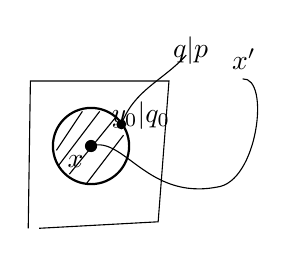
\begin{tikzpicture}[x=0.55cm,y=0.55cm]
\draw (0,0)--(0.05,3.4)--(3.25,3.4)--(3,0.15)--(0.25,0);
\draw[thick] (1.45,1.9) circle (0.88);
\draw (0.65,1.8)--(1.25,2.7) (0.7,1.45)--(1.65,2.7) (0.95,1.25)--(2.05,2.6) (1.35,1.04)--(2.2,2.15);
\fill (1.45,1.9) circle (2.2pt) (2.15,2.4) circle (1.8pt);
\node[below left] at (1.5,1.9) {$x$};
\draw (2.15,2.4).. controls (2.45,3.2) and (3.1,3.4)..(3.65,4.0);
\node at (3.75,4.1) {$\unsure{q|p}$};
\node at (2.6,2.6) {$\unsure{y_0|q_0}$};
\draw (1.45,1.9).. controls (2.2,2.15) and (2.75,0.65)..(4.35,0.95)
.. controls (5.3,1.05) and (5.6,3.5)..(4.95,3.45);
\node[above] at (4.98,3.45) {$x'$};
\end{tikzpicture}}

\uline{Th} $\forall x\in X$, $\exists$ une et une seule \deleted{\unsure{imm}}\inserted{imm.}
\unsure{ouverte|ouvert} analytique de $\widetilde X(x)$ dans
$T_x(X)$ dont a) l'image est un disque
b) l'application tangente en $\tilde x$
est l'identité.

\[
\pi_1(X,x)\underset{\unsure{j|?}}{\subset}G'\hookrightarrow G'_{\mathbb C}
\qquad \unsure{\mathcal U}
\]

\[
\begin{pmatrix}a&b\\c&d\end{pmatrix}.z=
\qquad
\begin{matrix}a\unsure{{}^{\ast}}&b\\-b&a\end{matrix}
\]

\[
\deleted{\unsure{alg|\deg}}\ \underline{P(x,q)}
\qquad Q_{\mathbb R}\qquad\text{\textcircled{\ensuremath{P_{\mathbb R}}}}\qquad
P(x,\rho\unsure{q})=P(x,x)\mathbin{\wedge}_{\operatorname{int}(\rho)}G'_{\mathbb C}
\]
\[
\begin{aligned}
P(x,\rho q)&=P(x,q)\mathbin{\wedge}_{\operatorname{int}(\rho)}G_{\mathbb C}\\
\unsure{q(q)|\rho}&\in\unsure{S'|S^1}\subset G'\subset G'_{\mathbb C}\\
&\mathbb C^{\ast}\quad Q_{\mathbb C}
\end{aligned}
\]
\diagram{\begin{tikzcd}[ampersand replacement=\&,row sep=small]
S_{\mathbb R}\arrow[r,phantom,"\subset" description]\arrow[d,phantom,"\cap" description] \& G'_{\mathbb R}\arrow[d,phantom,"\cap" description] \& {}\\
S_{\mathbb C}\arrow[r,phantom,"\subset" description] \& G'_{\mathbb C} \& P_{\mathbb C}
\end{tikzcd}}

\diagram{\begin{tikzcd}[ampersand replacement=\&,row sep=small]
P(x,q)\arrow[d,"\unsure{2}"'] \& G'_{\mathbb C}\arrow[d,"{\operatorname{int}(\unsure{\theta|\rho})}"]\\
P(x,x') \& G'_{\mathbb C}
\end{tikzcd}}

\[
E\longrightarrow E\otimes\Omega
\]
\figure{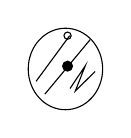
\begin{tikzpicture}[x=0.45cm,y=0.45cm]
\draw (0,0) ellipse (1.05 and 1.15);
\draw (-0.83,-0.35)--(0.12,0.94) (-0.58,-0.71)--(0.7,0.83)
(0.13,-0.55)--(0.56,0.09)--(0.28,-0.62)--(0.84,-0.07);
\fill (0.06,0.08) circle (2pt);\draw (0.06,0.94) circle (1.3pt);
\end{tikzpicture}}
\[
E\longrightarrow E\otimes\Omega
\]

\diagram{\begin{tikzcd}[ampersand replacement=\&,row sep=tiny]
\mathbb C^{\ast}=\operatorname{GL}(2,\mathbb R)\arrow[d]\\
\operatorname{GL}(2,\mathbb C)
\end{tikzcd}}

a) fibré inversible : $\underline{\Omega^{-1}}$\qquad
$\mathbb G_m\longrightarrow\operatorname{GP}_{\unsure{k|\mathbb C}}$

b) \deleted{fibré}\inserted{un} $\mathrm P(\Omega^{-1}+\Omega)$ avec
conn. intégrable

\[
\begin{pmatrix}\Omega&0\\\Omega^3&\Omega\end{pmatrix}
\]

\fbox{\parbox{0.65\linewidth}{Trouver une connexion intégrable
(alg) canonique sur
\[
\mathrm P(\Omega^{-1}+\Omega)=\overline{\mathrm V(\Omega^2)}
\]}}

\[
\begin{aligned}
\Omega^{-1}\oplus\Omega&\longrightarrow(\Omega^{-1}\oplus\Omega)\otimes\Omega\\
&=\Omega_X^0+\Omega^2.
\end{aligned}
\qquad (D,\omega)=(\unsure{d},\infty,\Delta)
\]
